\section{Definition von SIEN}

\gls{SIEM} ist das Ergebnis von der Kombination zwischen \glsfirst{SEM} und \glsfirst{SIM}. Das erste bezieht auf der Identifizierung, Sammlung, Beobachtung und Bericht Sicherheitsvorfälle mithilfe von verschiedenen Logdateien\citp{techopedia_SEM}. Das zweite ist ein Software, der bei der automatischen Sammlung von Loginformationen aus vielen Quellen, wie Firewall und Servers, untersützt \cite{techopedia_SIM}.

Um diese obengenannten Ziele zu erreichen, verwenden wir folgenden Methode:

\begin{itemize}[noitemsep]
   \item Was ist SIEN in der Literatur?
   \item State of Art the Art
   \item kurzer Vergleich zwsichen \textit{\gls{Proprietary}} und \gls{Open Source} Lösungen
   \item Existierende Rechecher über das Thema
\end{itemize}


- Architektur %https://www.spiceworks.com/it-security/vulnerability-management/articles/what-is-siem/
\begin{figure}[H]
   \centering
   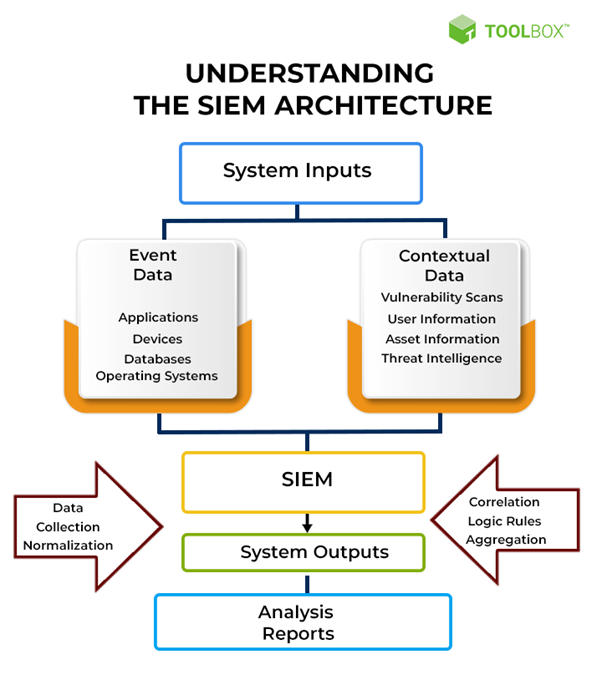
\includegraphics[width=0.8\textwidth]{assets/2_p1.png}
   \caption{Allgemeine Informationsfluss von \gls{SIEM} \\Quelle: \citep{Mohanan_What} }
   \centering
\end{figure}

- Anpassung %file:///C:/Users/bruno/Downloads/Security_Information_and_Event_Management_SIEM_Ana.pdf

\begin{figure}[H]
   \centering
   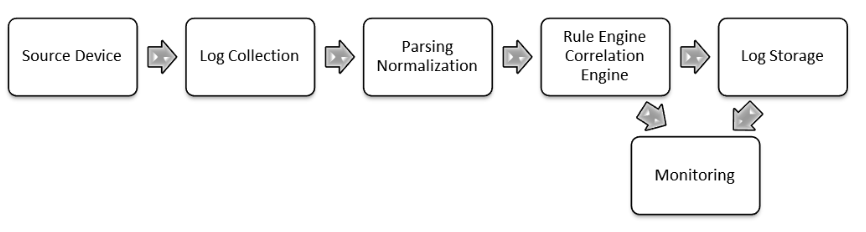
\includegraphics[width=0.8\textwidth]{assets/2_p2.png}
   \caption{Allgemeine Informationsfluss von \gls{SIEM} \\Quelle: \citep{Granadillo_SIEM} }
   \centering
\end{figure}







